\documentclass[10pt,a4paper]{report}
\usepackage[utf8]{inputenc}
\usepackage[russian]{babel}
\usepackage{amsmath}
\usepackage{amsfonts}
\usepackage{amssymb}
\usepackage{graphicx}
\renewcommand{\thesection}{\arabic{section}}
\setcounter{totalnumber}{10}
\setcounter{topnumber}{10}
\setcounter{bottomnumber}{10}
\renewcommand{\topfraction}{1}
\renewcommand{\textfraction}{0}
\author{Никитина Анна}
\title{Лабораторная работа №3.\\
	Программа для шифрования и подписи GPG, пакет Gpg4win}
\begin{document}
\maketitle
\tableofcontents
\pagebreak

\section{Цель работы}
Научиться создавать сертификаты, шифровать файлы и ставить ЭЦП.
\section{Описание работы}
Шифрование — обратимое преобразование информации в целях сокрытия от неавторизованных лиц, с предоставлением, в это же время, авторизованным пользователям доступа к ней. Одним из способов шифрования является ЭЦП.  \\
Электронная цифровая подпись (ЭЦП) — реквизит электронного документа, полученный в результате криптографического преобразования информации с использованием закрытого ключа подписи и позволяющий проверить отсутствие искажения информации в электронном документе с момента формирования подписи (целостность), принадлежность подписи владельцу сертификата ключа подписи (авторство), а в случае успешной проверки подтвердить факт подписания электронного документа (неотказуемость).  \\
При выполнении лабораторной работы для шифрования и создания ЭЦП используется пакет
Gpg4win. Он включает в себя:
\begin{itemize}
\item версию GnuPG — свободная программа для шифрования информации и создания электронных цифровых подписей;
\item Kleopatra (менеджер сертификатов для OpenPGP и X.509);
\item GPA (альтернативный менеджер сертификатов (GNU) для OpenPGP и X.509);
\item другие компоненты.
\end{itemize}
\pagebreak
\section{Ход работы}
Дальнейшие действия будут выполнены в графической оболочке \textbf{"Kleopatra"}.
\subsection{Создание  ключевой пары openPGP}
Для создания новой ключевой пары OpenPGP выполним команду \textit{"File -> New Certificate"}. После чего необходимо ввести персональную информацию: имя сертификата, адрес электронной почты пользователя (рисунок \ref{ris:image1} ).
\begin{figure}[ht]	\center{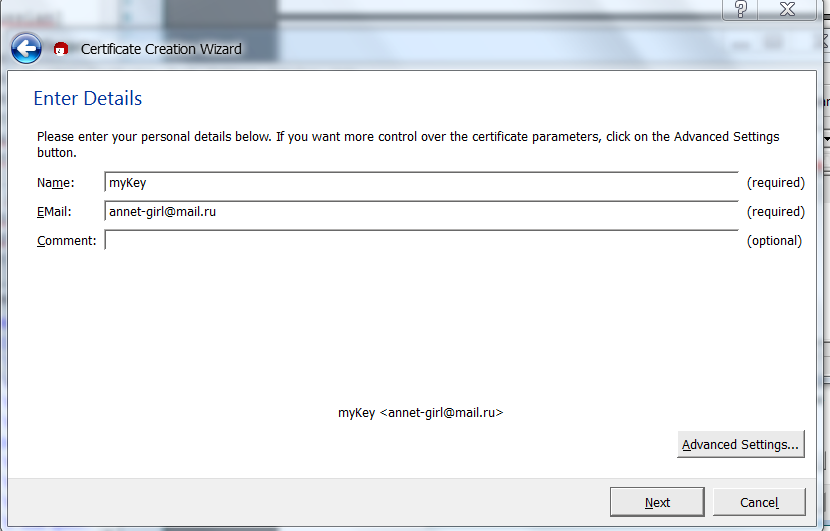
\includegraphics[width=0.8\linewidth]{image/1}}
\caption{Окно для ввода персональных данных.}\label{ris:image1}
\end{figure}

Далее подтвердим персональные данные, нажав кнопку \textit{"Create Key"} (рисунок \ref{ris:image2} ).
\begin{figure}[ht]	\center{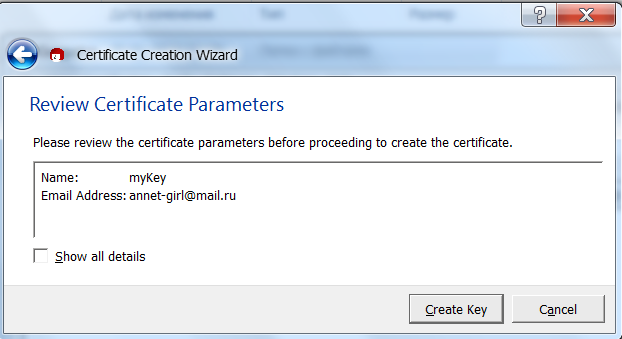
\includegraphics[width=0.8\linewidth]{image/2}}
\caption{Окно создания ключа.}
\label{ris:image2}
\end{figure}

После необходимо дважды ввести фразу-пароль (рисунок \ref{ris:image3} ).

\begin{figure}[h]
\parbox[b]{0.3\linewidth}
{\centering
    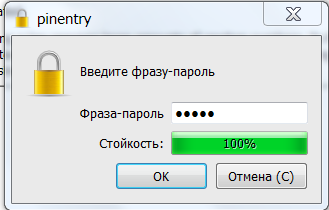
\includegraphics{image/3}}
\hspace*{\fill}
\parbox[b]{0.3\linewidth}
{\centering
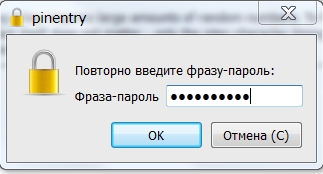
\includegraphics{image/4}}
 \caption{Окно ввода и подтверждения фразы-пароля}
\label{ris:image3}
\end{figure}

Сертификат успешно создан (рисунок  \ref{ris:image4} ).
\begin{figure}[h]
\center{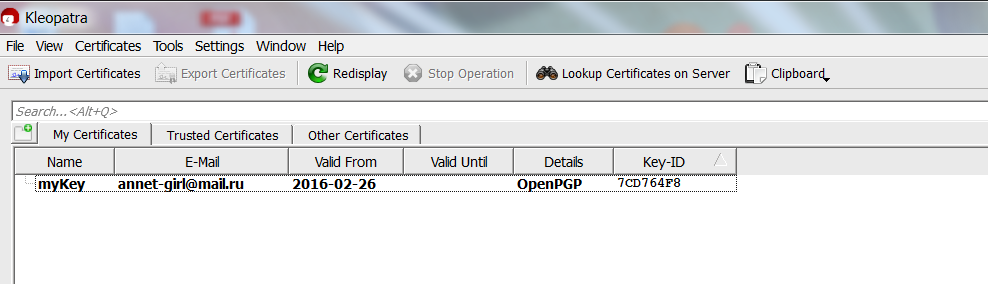
\includegraphics[width=1\linewidth]{image/5}}
\caption{Созданный сертификат}
\label{ris:image4}
\end{figure}

\subsection{Экспорт сертификата}
Для экспорта сертификата выполним команду \textit{"File ->  Export Certificate"}. После чего введем имя файла \textit{key.asc} (рисунок \ref{ris:image5} ).
\begin{figure}[h]
\center{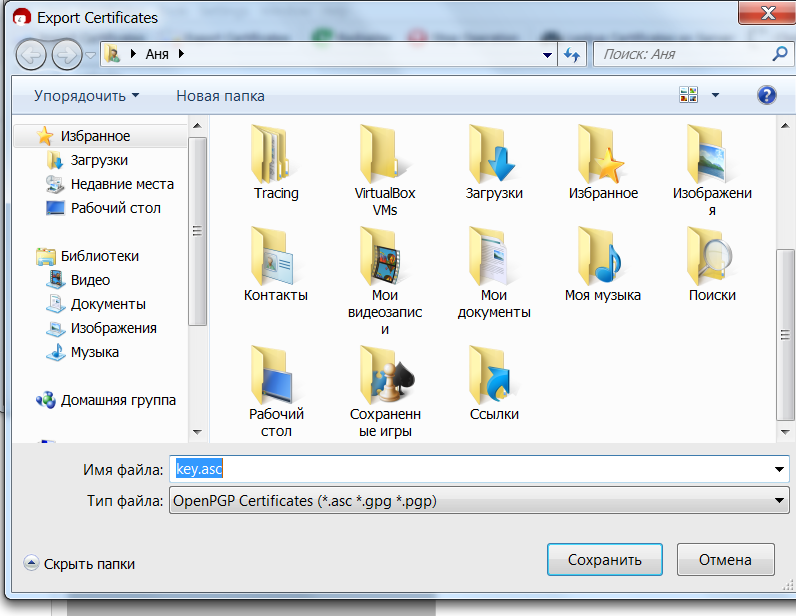
\includegraphics[width=0.7\linewidth]{image/6}}
\caption{Экспорт сертификата}
\label{ris:image5}
\end{figure}

\subsection{Поставить ЭЦП на файл}
Для того, что бы поставить ЭЦП на файл выполним команду \textit{"File -> Sign/Encrypt Files"} и выберем файл, на который необходимо поставить ЭЦП.В нашем случае это \textit{1.PNG} (рисунок \ref{ris:image6} ).
\begin{figure}[h]
\center{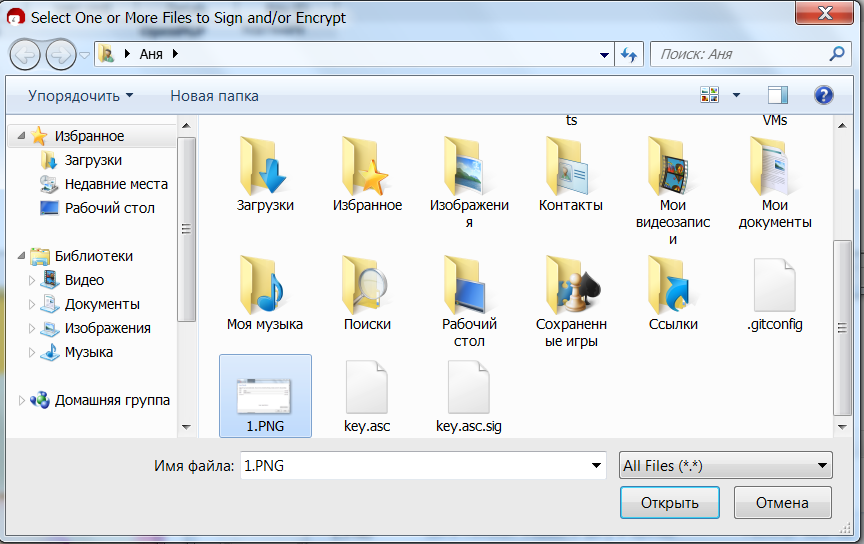
\includegraphics[width=0.6\linewidth]{image/7}}
\caption {Выбор файла}
\label{ris:image6}
\end{figure}

После выберем одно из трех предложенных действий.
\begin{itemize}
\item Sign and Encrypt
\item Encrypt
\item Sign
\end{itemize} 
В нашем случае \textit{Sign} - создание цифровой подписи (рисунок \ref{ris:image7} ).
\begin{figure}[h]
\center{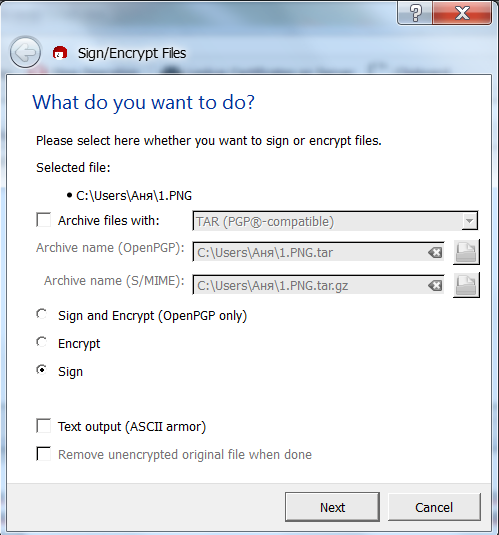
\includegraphics[width=0.6\linewidth]{image/8}}
\caption{Поставить ЭЦП на файл}
\label{ris:image7}
\end{figure}

Выберем для подписи стандарт OpenPGP и сертификат, созданный ранее (рисунок \ref{ris:image8} ).
\begin{figure}[h]	\center{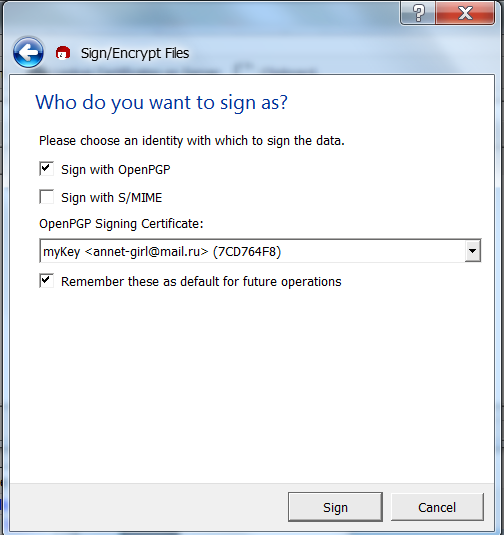
\includegraphics[width=0.8\linewidth]{image/9}}
\caption{Выбор стандарта и сертификата для ЭЦП}
\label{ris:image8}
\end{figure}

Введем пароль (рисунок \ref{ris:image9} ).
\begin{figure}[h]
\center{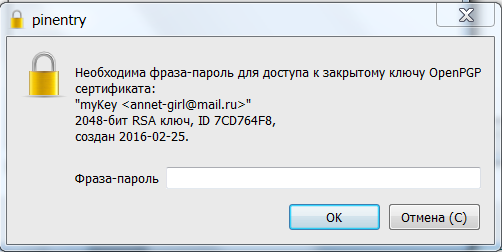
\includegraphics[width=1\linewidth]{image/10}}
\caption{Ввод пароля}
\label{ris:image9}
\end{figure}

Видим сообщение об успешном создании подписи на файл \textit{1.PNG}, новый подписаннный файл называется \textit{1.PNG.sig} (рисунок \ref{ris:image10} ).
\begin{figure}[h]	\center{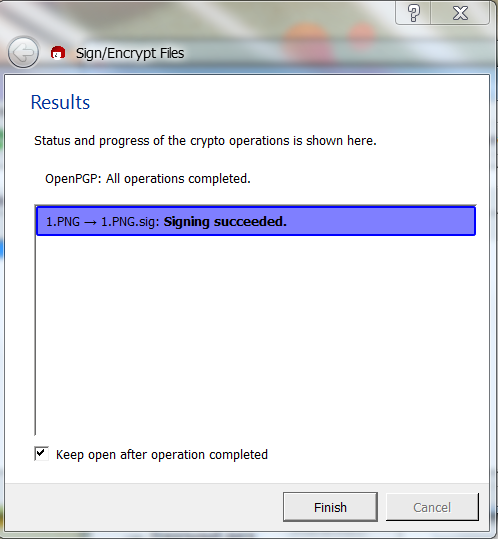
\includegraphics[width=0.8\linewidth]{image/11}}
\caption{Успешная подпись файла}
\label{ris:image10}
\end{figure}

\subsection{Импорт сертификата и его подпись}
Для импорта сертификата выполним команду \textit{File -> Import Certificates} и выберем необходимый файл типа \textit{.asc} (рисунок \ref{ris:image11} ).
\begin{figure}[h]	\center{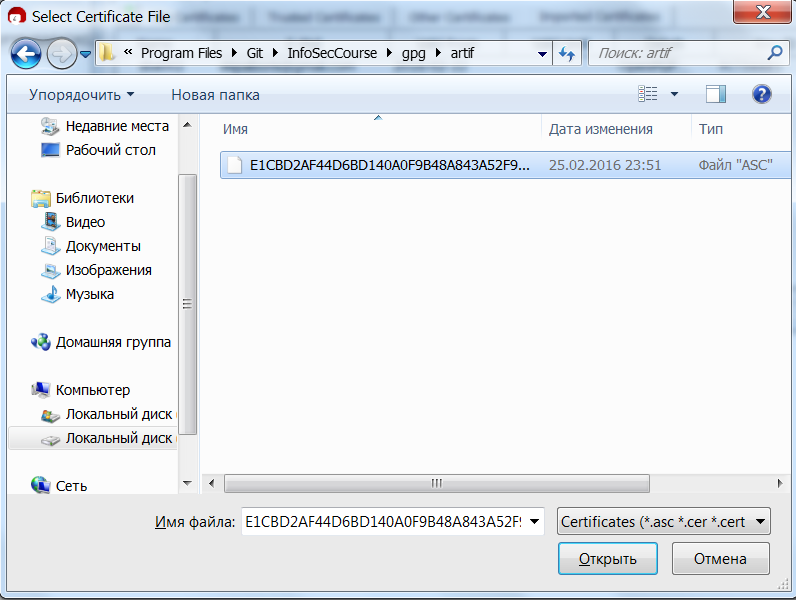
\includegraphics[width=0.5\linewidth]{image/12}}
\caption{Выбор файла для импорта}
\label{ris:image11}
\end{figure}

После чего импортированный сертификат появится в рабочем пространстве (рисунок \ref{ris:image12} ).
\begin{figure}[h]	\center{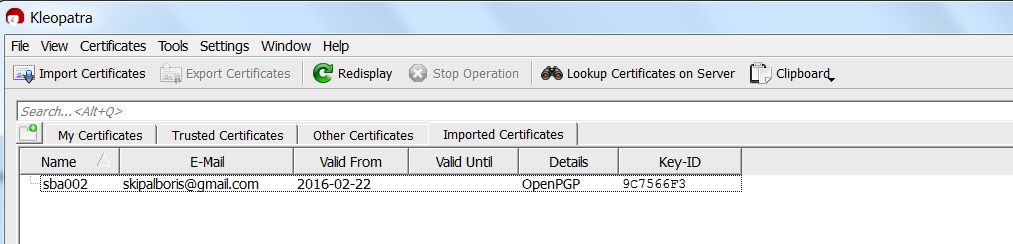
\includegraphics[width=0.8\linewidth]{image/13}}
\caption{Успешный импорт сертификата}
\label{ris:image12}
\end{figure}

Подпишем его, как это было описано выше (рисунок \ref{ris:image13} ).
\begin{figure}[h]	\center{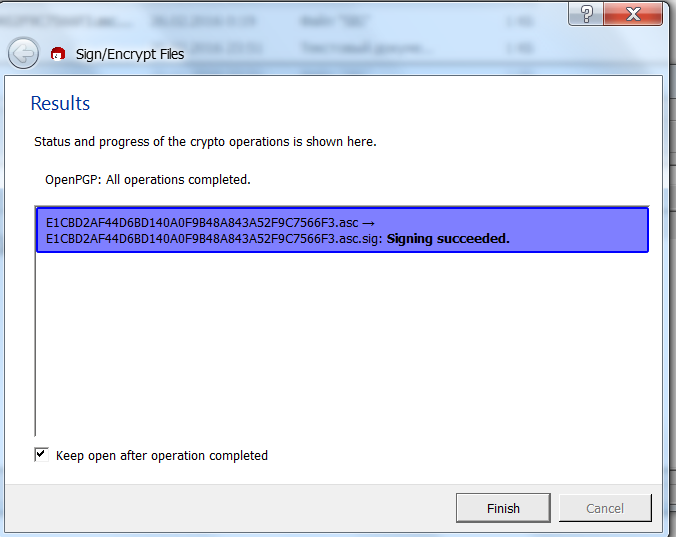
\includegraphics[width=0.7\linewidth]{image/14}}
\caption{Подпись импортированного сертификата }
\label{ris:image13}
\end{figure}

Для проверки воспользуемся командой \textit{File -> Decrypt/Verify Files} и выберем подписанный ранее сертификат типа \textit{.asc/sig} (рисунок \ref{ris:image14} ).
\begin{figure}[h]	\center{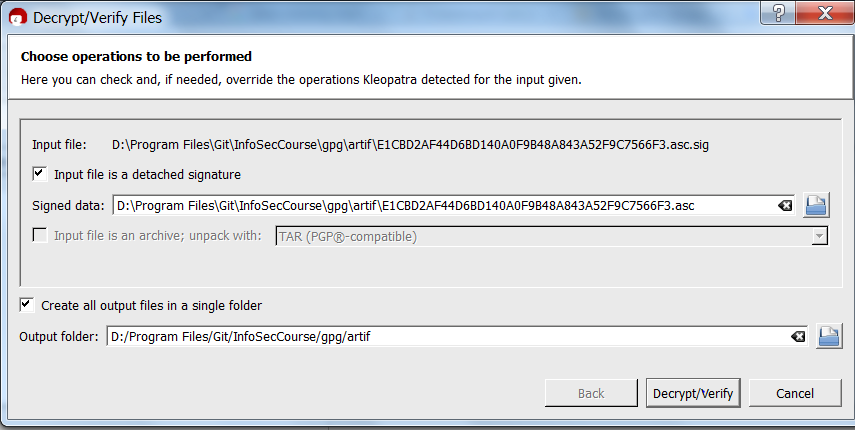
\includegraphics[width=0.8\linewidth]{image/20}}
\caption{Проверка подписи}
\label{ris:image14}
\end{figure}

Проверка показывает, кем была осуществлена подпись (рисунок \ref{ris:image15}).
\begin{figure}[h]	\center{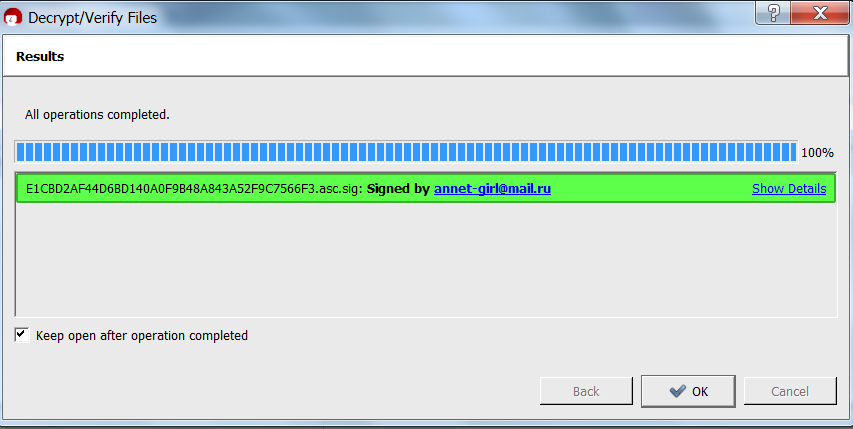
\includegraphics[width=0.7\linewidth]{image/21}}
\caption{Проверка подписи}
\label{ris:image15}
\end{figure}
\subsection{Работа с чужим сертификатом}

С помощью чужого сертификата зашифруем и подпишем какой-либо документ, например файл \textit{Боря.txt}.  В свою очередь коллега, кторому принадлежит этот сертификат, расшифрует переданный документ \textit{Боря.txt.gpg}, используя свой пароль. \\
Проделаем действия в другую сторону. Коллега с помощью моего ключа зашифровал документ и передал его мне \textit{Ann.txt.gpg}. Командой \textit{File -> Decrypt/Verify Files} расшифруем документ. После ввода верного пароля видим окно с сообщением об удачном расшифровании файла. 
(рисунок \ref{ris:image16} ), также появился файл \textit{Ann.txt}, который можно прочитать. 
\begin{figure}[h]	\center{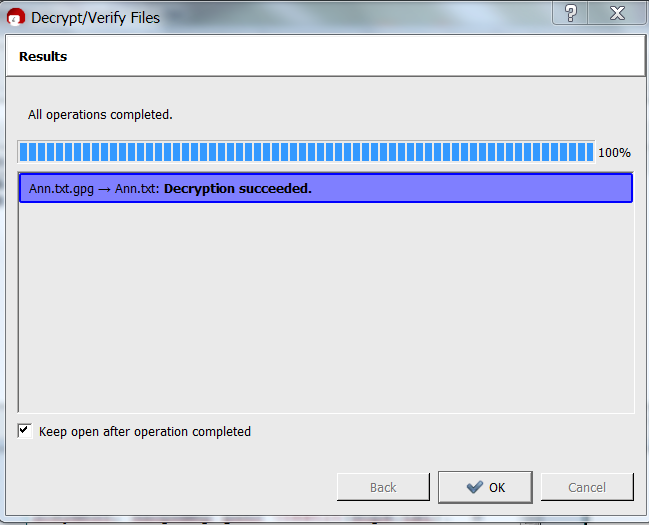
\includegraphics[width=0.7\linewidth]{image/22}}
\caption{Успешное расшифрование файла}
\label{ris:image16}
\end{figure}

\subsection{Использование GNU Privacy handbook}
С помощью GNU Privacy handbook проделаем некоторые действия по использованию gpg через командную строку. \\
Для создания ключевой пары введем в консоле команду \textit{gpg --gen-key}. Далее выберем тип ключа, его размер, срок действия, укажем ID пользователя, электронную почту, введем пароль, после чего создастся ключевая пара. Полный лог вышеперечисленных действий приведен в файле \textit{log.txt}. \\
Создали ключ типа RSA и DSA, размером 1024, срок действия которого не ограничен. \\
 
Для создания сертификата воспользуемся командой \textit{gpg --output key\_console.asc  --gen-revoke anna\_nik}, в которой укажем выходной файл сертификата и ключевую пару. После ответа на необходимые вопросы сертификат будет создан (рисунок \ref{ris:image17} ). 
\begin{figure}[h]	\center{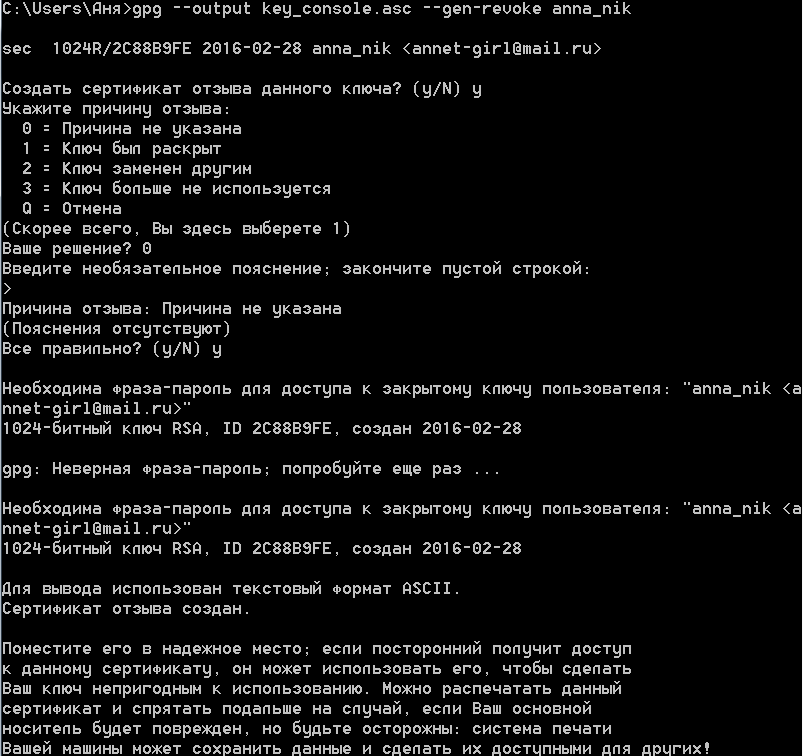
\includegraphics[width=0.8\linewidth]{image/18}}
\caption{Создание сертификата}
\label{ris:image17}
\end{figure}

Для просмотра списка созданных ключей введем команду \textit{gpg --list-key}. Видим в списке все ключи, созданные или импортированные как в графической оболочке, так и в консоле (рисунок \ref{ris:image18} ).
\begin{figure}[h]
\center{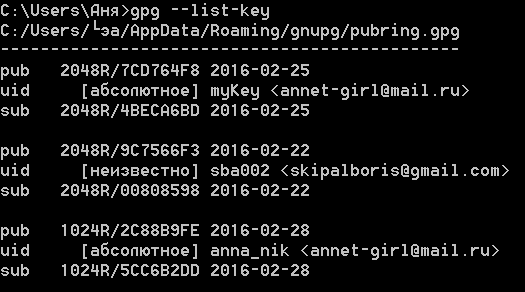
\includegraphics[width=0.8\linewidth]{image/17}}
\caption{Список созданных ключей}
\label{ris:image18}
\end{figure}

Для того, чтобы отправить свой открытый ключ корреспонденту необходимо его экспортировать командой  \textit{gpg --output anna\_nik.gpg --export anna\_nik}.  

Для подписи документа используем команду \textit{gpg --output 2.PNG.sin --sign 2.PNG}. После ввода пароля создается новый полписанный документ \textit{2.PNG.sin} (рисунок \ref{ris:image19} ).
\begin{figure}[h]	\center{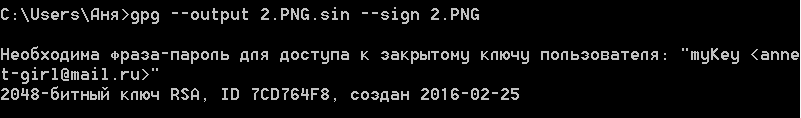
\includegraphics[width=0.8\linewidth]{image/19}}
\caption{Подпись документа}
\label{ris:image19}
\end{figure}

\section{Вывод}
В ходе лабораторной работы, используя пакет Gpg4win, я научилась создавать собственные ключевые пары и сертификаты на них; подписывать файлы и проверять подпись, а также зашифровывать и расшифровывать документы с помощью собственного сертификата или стороннего. Вышеперечисленные действия легко произвести как из графической обочки \textbf{Kleopatra}, так и из командной строки. 
\end{document}